%%%%%%%%%%%%%%%%%%%%%%%%%%%%%%%%%%%%%%%%%
% Class Notes Template
% LaTeX Template
% By: Ryan Grove
%%%%%%%%%%%%%%%%%%%%%%%%%%%%%%%%%%%%%%%%%

%----------------------------------------------------------------------------------------
%	PACKAGES AND OTHER DOCUMENT CONFIGURATIONS
%----------------------------------------------------------------------------------------

\documentclass[paper=a4, fontsize=11pt]{scrartcl} % A4 paper and 11pt font size

\usepackage[T1]{fontenc} % Use 8-bit encoding that has 256 glyphs
\usepackage{fourier} % Use the Adobe Utopia font for the document - comment this line to return to the LaTeX default
\usepackage[english]{babel} % English language/hyphenation
\usepackage{amsmath,amsfonts,amsthm} % Math packages

\usepackage{lipsum} % Used for inserting dummy 'Lorem ipsum' text into the template

\usepackage{sectsty} % Allows customizing section commands
\allsectionsfont{\centering \normalfont\scshape} % Make all sections centered, the default font and small caps

\usepackage{fancyhdr} % Custom headers and footers
\pagestyle{fancyplain} % Makes all pages in the document conform to the custom headers and footers
\fancyhead{} % No page header - if you want one, create it in the same way as the footers below
\fancyfoot[L]{} % Empty left footer
\fancyfoot[C]{} % Empty center footer
%\fancyfoot[R]{\thepage} % Page numbering for right footer
\renewcommand{\headrulewidth}{0pt} % Remove header underlines
\renewcommand{\footrulewidth}{0pt} % Remove footer underlines
\setlength{\headheight}{13.6pt} % Customize the height of the header

\numberwithin{equation}{section} % Number equations within sections (i.e. 1.1, 1.2, 2.1, 2.2 instead of 1, 2, 3, 4)
\numberwithin{figure}{section} % Number figures within sections (i.e. 1.1, 1.2, 2.1, 2.2 instead of 1, 2, 3, 4)
\numberwithin{table}{section} % Number tables within sections (i.e. 1.1, 1.2, 2.1, 2.2 instead of 1, 2, 3, 4)

\setlength\parindent{0pt} % Removes all indentation from paragraphs - comment this line for an assignment with lots of text

\usepackage{lastpage}
\usepackage{fancyhdr}
\cfoot{\thepage\ of \pageref{LastPage}}

\def\v{\hbox{$\mathbf v$}}
\def\w{\hbox{$\mathbf w$}}
\def\u{\hbox{$\mathbf u$}}
\def\x{\hbox{$\textbf{x}$}}
\def\z{\hbox{$\mathbf z$}}
\def\a{\hbox{$\mathbf a$}}
\def\b{\hbox{$\mathbf b$}}
\def\L{\hbox{$\mathcal L$}}
\def\C{\hbox{$\mathbb C$}}
\def\B{\hbox{$\mathcal B$}}
\def\R{\hbox{$\mathbb R$}}
\def\X{\hbox{$\underline X$}}
\def\Q{\hbox{$\mathbb Q$}}
\def\R{\hbox{$\mathbb R$}}
\def\N{\hbox{$\mathbb N$}}
\def\C{\hbox{$\mathbb C$}}
\def\0{\hbox{$\mathbf 0$}}
\def\Y{\hbox{$\underline Y$}}
\def\a{\hbox{$\mathbf a$}}
\def\u{\hbox{$\mathbf u$}}
\def\w{\hbox{$\mathbf w$}}
\def\y{\hbox{$\mathbf y$}}
\def\X{\hbox{$\underline X$}}
\def\dd{\hbox{$\partial $}}
\def\B{\hbox{$\mathcal B$}}
\def\F{\hbox{$\mathcal F$}}
\def\L{\hbox{$\mathcal L$}}
\def\M{\hbox{$\mathcal M$}}
\def\D{\hbox{$\mathscr {D}$}}
\def\RR{\hbox{$\mathscr{R}$}}
\def\I{\hbox{$\mathcal I$}}

\usepackage{amssymb}
%\theoremstyle{plain}
\usepackage[margin = .75in]{geometry}
\newtheorem{claim}{Claim}
\newtheorem{theorem}{Theorem}[section]
\newtheorem{lemma}[theorem]{Lemma}
\newtheorem{proposition}[theorem]{Proposition}
\newtheorem{corollary}[theorem]{Corollary}
\newtheorem{problem}[theorem]{Problem}
%\theoremstyle{definition}
\newtheorem{definition}[theorem]{Definition}
%\theoremstyle{remark}
\newtheorem{remark}[theorem]{Remark}
\newtheorem{remarks}[theorem]{Remarks}
\newtheorem{example}[theorem]{Example}
\newcommand{\ds}{\displaystyle}
\newcommand{\ZZ}{\mathbb{Z}}
\newcommand{\QQ}{\mathbb{Q}}
\newcommand{\e}{\varepsilon}
\newcommand{\bbf}{\textbf}
\newcommand{\p}{\parallel}
\usepackage{color}
\newcommand{\field}[1]{\mathbb{#1}}
\usepackage{amsmath}
\usepackage{amsthm}
\usepackage{amssymb}
\usepackage{mathrsfs}
\usepackage{cancel}
\usepackage{upgreek}
\usepackage{graphicx}
\usepackage{multirow}
\usepackage{setspace}
\usepackage{url}
\usepackage{subfigure}
\usepackage{enumerate}
\usepackage{cases}
\usepackage{mathrsfs}
\usepackage{rotating}

%----------------------------------------------------------------------------------------
%	TITLE SECTION
%----------------------------------------------------------------------------------------

\newcommand{\horrule}[1]{\rule{\linewidth}{#1}} % Create horizontal rule command with 1 argument of height

\title{	
\normalfont \normalsize 
\textsc{Ryan Grove, Clemson University, MATH1080 - 9} \\ [25pt] % Your name, university, class
\horrule{0.5pt} \\[0.4cm] % Thin top horizontal rule
\huge Section 10.2: Calculus with Parametic Curves\\ % The assignment title
\horrule{2pt} \\[0.5cm] % Thick bottom horizontal rule
}

\author{Date:} % The due date

\date{\normalsize April 5, 2016} % A custom date

\begin{document}

\maketitle % Print the title

\begin{flushleft}
\begin{tabular}{l l}
Name: \rule{3.2in}{.01cm}  & {}%Table number: \rule{1in}{.01cm}\\
\end{tabular}
\end{flushleft}

%----------------------------------------------------------------------------------------
%	Lecture
%----------------------------------------------------------------------------------------

\section*{\textbf{Lecture:}}
\indent

Having seen how to represent curves by parametric equations, we now apply the methods of calculus to these parametric curves. In particular, we solve problems involving tangents, area, arc length, and surface area.\\

\section*{Tangents}
Suppose $f$ and $g$ are differentiable functions and we want to find the tangent line at a point on the curve $x=f(t)$, $y=g(t)$ where $y$ is also a differentiable function of $x$. Then the Chain Rule gives

\[\ds\frac{dy}{dt} = \ds\frac{dy}{dx}\cdot \ds\frac{dx}{dt}\]
\indent

If \text{ }$\ds\frac{dx}{dt}\neq 0$, we solve for $\ds\frac{dy}{dx}$:\\
\indent\\

\[\boxed{\quad \ds\frac{dy}{dx} = \ds\frac{\text{ }\text{ }\ds\frac{dy}{dt}\text{ }\text{ }}{\ds\frac{dx}{dt}} \quad \text{ if } \text{ } \ds\frac{dx}{dt}\neq 0 \quad} \quad \quad \quad \quad (1)\]
\indent\\
\indent\\
\indent

Equation (1) enables us to find the slope $\ds\frac{dy}{dx}$ of the tangent to a parametric curve without having to eliminate the parameter $t$ (that is, without having to write it as a Cartesian Equation). From equation (1) we see that a curve has a horizontal tangent when $\ds\frac{dy}{dt}=0$ (provided that $\ds\frac{dx}{dt}\neq 0$) and it has a vertical tangent when $\ds\frac{dx}{dt}=0$ (provided that $\ds\frac{dy}{dt}\neq 0$). This information is useful for sketching parametric curves.\\
\indent\\
\indent

We can also find $\ds\frac{d^2 y}{dx^2}$ by replacing $y$ in Equation (1) by $\ds\frac{dy}{dx}$:\\
\indent\\
\indent

\[\ds\frac{d^2 y}{dx^2} = \ds\frac{d}{dx} \left(\ds\frac{dy}{dx}\right) = \ds\frac{\ds\frac{d}{dt}\left(\ds\frac{dy}{dx}\right)}{\ds\frac{dx}{dt}}\]
\indent

\newpage
\underline{Example 1}: A curve $C$ is defined by the parametric equations $x=t^2$, $y=t^3-3t$.\\
\begin{itemize}
\item[(a)] Show that $C$ has two tangents at the point $(3,0)$ and find their equations.\\
\item[(b)] Find the points on $C$ where the tangent is horizontal or vertical.\\
\item[(c)] Determine where the curve is concave upward or downward.\\
\item[(d)] Sketch the curve.\\
\end{itemize}
\indent

SOLUTION:
\begin{itemize}
\item[(a)] \text{ }
\vspace{1.8in}
\item[(b)] \text{ }
\vspace{1.5in}
\item[(c)] \text{ }
\vspace{1.5in}
\item[(d)] \text{ }
\vspace{1.5in}
\end{itemize}
 \indent
 
 \newpage
 
 \underline{Example 2}:
 \begin{itemize}
 \item[(a)] Find the tangent to the cycloid $x=r(\theta - \sin\theta), y=r(1-\cos\theta)$ at the point where $\theta = \ds\frac{\pi}{3}$.\\
 \item[(b)] At what points is the tangent horizontal? When is it vertical?\\
 \end{itemize}
 \indent
 
 SOLUTION:\\
 \begin{itemize}
 \item[(a)] \text{ }
 \vspace{2.8in}
 \[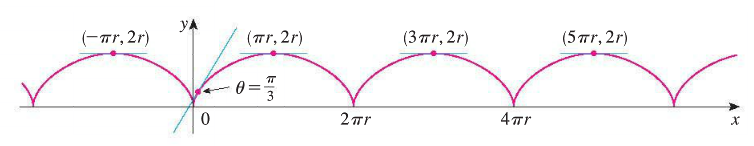
\includegraphics[scale=0.55]{10-2pic1.png}\]
 \item[(b)] \text{ }
 \vspace{3.4in}
 \end{itemize}
 
 \section*{Areas}
 
 We know the area under a curve $y=f(x)$ from $a$ to $b$ is $A=\ds\int_a^b f(x)dx$, where $f(x)\geq 0$. If the curve is traced out once by the parametric equations $x=f(t)$ and $y=g(t)$, $\alpha \leq t \leq \beta$, then we can calculate an area formula by using the Substitution Rule for Definite Integrals as follows:
 
 \[\boxed{ \quad A = \ds\int_a^b y dx = \ds\int_\alpha^\beta g(t)f'(t)dt \quad }\]
 \indent\\
 \indent
 
 \underline{Example 3}: Find the area under one arch of the cycloid
 \[x=r(\theta - \sin\theta) \quad y=r(1-\cos\theta)\]
 
 SOLUTION:\\
 
 \vspace{3.5in}
 
 \newpage
 \section*{Arc Length}
 We already know how to find the length $L$ of a curve $C$ given in the form $y=f(x)$, $a\leq x\leq b$. As long as $f'$ is continuous we have\\
 
 \[L=\ds\int_a^b \ds\sqrt{1+\left(\ds\frac{dy}{dx}\right)^2}dx \quad \quad \quad \quad (2)\]
 \indent
 
 Suppose that $C$ can also be described by the parametric equations $x=f(t)$ and $y=g(t)$, $\alpha\leq t\leq \beta$, where $\ds\frac{dx}{dt}=f'(t)>0$. This means that $C$ is traversed once, from left to right, as $t$ increases from $\alpha$ to $\beta$ and $f(\alpha)=a, f(\beta)=b$. Putting Equation (1) into Formula (2) and using the Substitution Rule, we obtain\\
 
 \[L=\ds\int_a^b\ds\sqrt{1+\left(\ds\frac{dy}{dx}\right)^2}dx = \ds\int_\alpha^\beta\ds\sqrt{1+\left(\ds\frac{dy/dt}{dx/dt}\right)^2}\ds\frac{dx}{dt}dt.\]
 \indent
 
 Since $\ds\frac{dx}{dt}>0$, we have\\
 
 \[L = \ds\int_\alpha^\beta \ds\sqrt{\left(\ds\frac{dx}{dt}\right)^2 + \left(\ds\frac{dy}{dt}\right)^2}dt \quad \quad  \quad \quad (3)\]
 \indent
 
 Even if $C$ can't be expressed in the form $y=f(x)$, Formula (3) is still valid but we obtain it by polygonal approximations. (Derivation eliminated here but is shown in 10.2, page 648, of the textbook).\\
 \indent\\
 \indent
 
 \fbox{
  \parbox{\textwidth}{
  \vspace{5pt} \textbf{\underline{Theorem 5}}: If a curve $C$ is described by the parametric equations $x=f(t), y=g(t), \alpha\leq t \leq \beta$, where $f'$ and $g'$ are continuous on $[\alpha,\beta]$ and $C$ is traversed exactly once as $t$ increases from $\alpha$ to $\beta$, then the length of $C$ is\\
  \indent
  
  \[L=\ds\int_\alpha^\beta \ds\sqrt{\left(\ds\frac{dx}{dt}\right)^2 + \left(\ds\frac{dy}{dt}\right)^2}dt\]
  \indent\\
  \indent
  
  }}
  \indent\\
  \indent
  
  \newpage
  \underline{Example 4}: If we use the representation of the unit circle given in Example 2 in Section 10.2,
  \[x=\cos t \quad y=\sin t \quad 0\leq t \leq 2\pi\]
  
 then $\ds\frac{dx}{dt}=\underline{\hspace{1in}}$ and $\ds\frac{dy}{dt}=\underline{\hspace{1in}}$, so Theorem 5 gives\\

\vspace{0.6in}

as expected. If, on the other hand, we use the representation given in Example 3 in Section 10.1, 
\[x=\sin 2t \quad y=\cos 2t \quad 0\leq t \leq 2\pi\]
then $\ds\frac{dx}{dt} = \underline{\hspace{1in}}$, $\ds\frac{dy}{dt}=\underline{\hspace{1in}}$, and the integral in Theorem 5 gives\\

\vspace{0.6in}
\indent

*Notice that the latter integral gives \underline{twice} the arc length of the circle because as $t$ increases from $0$ to $2\pi$, the point $(\sin 2t,\cos 2t)$ traverses the circle \underline{twice}. In general, when find the length of a curve $C$ from a parametric representation, be careful that $C$ is traversed only \underline{once} within the bounds you are integrating over.\\
\indent

\underline{Example 5}: Find the length of one arch of the cycloid
\[x=r(\theta - \sin\theta), \quad y=r(1-\cos\theta).\]
\indent

SOLUTION:\\

\vspace{3.5in}
\newpage
\section*{Surface Area}
In the same way as for arc length we can adapt our surface area formula for parametric equations. Consider the curve given by parametric equations $x=f(t), y=g(t), \alpha\leq t \leq \beta$, where $f',g'$ are continuous and $g(t)\geq 0$. The area of the surface that results by rotating the curve about the given specified axis is as follows:\\
\indent

Rotating about the $\mathbf{x-}$\textbf{axis}:
\[\boxed{\quad S = \ds\int_\alpha^\beta 2\pi y \ds\sqrt{\left(\ds\frac{dx}{dt}\right)^2 + \left(\ds\frac{dy}{dt}\right)^2}dt \quad }\]

Rotating about the $\mathbf{y-}$\textbf{axis}:
\[\boxed{\quad S = \ds\int_\alpha^\beta 2\pi x \ds\sqrt{\left(\ds\frac{dx}{dt}\right)^2 + \left(\ds\frac{dy}{dt}\right)^2}dt \quad }\]
\indent\\
\indent

\underline{Example 6}: Show that the surface area of a sphere of radius $r$ is $4\pi r^2$.\\
\indent

SOLUTION: The sphere is obtained by rotating the semicircle
\[x=r\cos t, \quad y=r\sin t, \quad 0 \leq t \leq \pi\]
about the $x-$axis.\\

\vspace{3in}

 

%\fbox{
%  \parbox{\textwidth}{
%  \vspace{5pt}


%----------------------------------------------------------------------------------------

\end{document}